\documentclass{article}
\usepackage{graphicx}
\usepackage{amsmath}
\usepackage{array}
\usepackage[font=small, labelfont={sf,bf}, margin=1cm]{caption}
\usepackage{tabularx}
\usepackage{amssymb}



\date{Due:Sep 19 Edit: \today}
\title{PHYS 225 HW 3}
\author{James Liu}

\begin{document}
\maketitle
\begin{itemize}
    \item [1.]
    \begin{itemize}
        \item [a)]
        \begin{itemize}
            \item [i:]
            \begin{align*}
                \begin{bmatrix}
                    ct\\
                    x
                \end{bmatrix}
                =\gamma\cdot\begin{bmatrix}
                     1&\beta\\\beta & 1
                \end{bmatrix}\begin{bmatrix}
                    ct'\\ x'
                \end{bmatrix}
            \end{align*}
            There will be 4 space time events. Define \(C_w\) as the west person claps similar with \(C_e\) being the event where east people clap.
            \(T_c\) be the event car traveling to the tree. \(W_c\) be the event that the car travels by the west person. \(S\) be the gound reference system and \(S'\) be the car's reference system.
            Build a cordinate system with \(t_0\) when the east people clap and \(x_0\) the location of East person. \(t_0'\) is when the car saw the east people clap with \(x_0'\) the position of east person in car's frame.
            Then it is easy that we can have this table:
            \begin{center}
                \begin{tabular}{ c c c c c}
                event & t & x & t' &x'\\ \hline
                \(C_e\) & 0&0&0&0 \\  
                \(C_w\) & 0&-L&?&? \\
                \(W_e\) &?&?&0&?\\
                \(T_c\) &?&?&?&?
                \end{tabular}
            \end{center}
            Now try find the event \(C_w\)'s space time coordinate in \(S'\):
            \begin{align*}
                \begin{bmatrix}
                    \frac{5}{3}&-\frac{4}{3}\\
                    -\frac{4}{3}&\frac{5}{3}
                \end{bmatrix}
                \begin{bmatrix}
                    0\\-L
                \end{bmatrix}=
                \begin{bmatrix}
                    \frac{4L}{3}\\
                    -\frac{5L}{3}
                \end{bmatrix}
            \end{align*}
            Then we can find car's position at  \(\frac{4L}{3c}\) in its own frame which the x value shall be the same to its start point:
            \[x'_c = -\frac{5}{3}L+\frac{4L}{3c}\times \frac{4}{5}c=-\frac{9}{15}L\]
            Then, the event having space time coordinate \(\begin{pmatrix}\frac{4L}{3c}\\-\frac{9}{15}L\end{pmatrix}\) in the ground reference frame would contain the location of the tree:
           \begin{align*}
            \begin{bmatrix}
                \frac{5}{3}&\frac{4}{3}\\
                \frac{4}{3}&\frac{5}{3}
            \end{bmatrix}
            \begin{bmatrix}\frac{4L}{3}\\-\frac{9}{15}L\end{bmatrix}=
            \begin{bmatrix}
                \frac{64}{45}L\\
                \frac{7}{9}L
            \end{bmatrix}
           \end{align*}
           Thus the location of the tree is \(\frac{7}{9}L\) east of the east person.
           and the table becomes:
           \begin{center}
            \begin{tabular}{ c c c c c}
            event & t & x & t' &x'\\ \hline
            \(C_e\) & 0&0&0&0 \\  
            \(C_w\) & 0&-L&\(\frac{4L}{3c}\)&\(-\frac{5L}{3}\) \\
            \(W_e\) &?&?&0&\(-\frac{9}{15}L\)\\
            \(T_c\) &\(\frac{64L}{45c}\)&\(\frac{7}{9}L\)&\(\frac{4L}{3c}\)&\(-\frac{9}{15}L\)
            \end{tabular}
            \end{center}
            \item [ii:] Setting the speed of car as \(kc\), then \(\gamma = \frac{1}{\sqrt{1-k^2}}\) and \(\beta = k\).
                        Thus, the space time event that the west people claps is still \(\begin{bmatrix}
                        0\\-L
                        \end{bmatrix}\). Then the space time even in car's frame is:
                        \begin{align*}
                            \begin{bmatrix}
                                \frac{1}{\sqrt{1-k^2}}&-\frac{k}{\sqrt{1-k^2}}\\
                                -\frac{k}{\sqrt{1-k^2}}&\frac{1}{\sqrt{1-k^2}}
                            \end{bmatrix}
                            \begin{bmatrix}
                                0\\-L
                            \end{bmatrix}=
                            \begin{pmatrix}
                                \frac{k}{\sqrt{1-k^2}}L\\ 
                                -\frac{1}{\sqrt{1-k^2}}L
                            \end{pmatrix}
                        \end{align*}
                        The car will locate at:
                        \begin{align*}
                            x'_c  =  \frac{k}{\sqrt{1-k^2}}\frac{L}{c}\times kc-\frac{1}{\sqrt{1-k^2}}L = \frac{k^2-1}{\sqrt{1-k^2}}L
                        \end{align*}
                        The tree event will be at:
                        \begin{align*}
                            \begin{bmatrix}
                                \frac{1}{\sqrt{1-k^2}}&\frac{k}{\sqrt{1-k^2}}\\
                                \frac{k}{\sqrt{1-k^2}}&\frac{1}{\sqrt{1-k^2}}
                            \end{bmatrix}
                            \begin{bmatrix}
                                \frac{k}{\sqrt{1-k^2}}L\\ \frac{k^2-1}{\sqrt{1-k^2}}L
                            \end{bmatrix}=
                            \begin{bmatrix}
                                \frac{k^3}{1-k^2}L \\ \frac{2k^2-1}{1-k^2}L
                            \end{bmatrix}
                        \end{align*}
                        set \(\frac{2k^2-1}{1-k^2}L = 0\), \(k = \frac{1}{\sqrt 2}\approx 70.7\%\).\\ Thus the velocity should be \(\frac{c}{\sqrt2}\)
                        Subsituting \(k = v/c\) we have tree's position in \(S\): \(x_{t} = \frac{2\frac{v^2}{c^2}-1}{1-\frac{v^2}{c^2}}\)
        
        \end{itemize}
        \newpage
        \item [b)] If the car is traveling form east then due to the rear clock ahead effect, the west people will clap first and left a tree marking that event on the same location if when the car travels to the west person when spoting the east person clap.
        As shown on graph, as either way, the red line must trverse the \([W_x,W_{t0}]\) point as in car's reference frame, it is at \([W_x]\) when east people claps.    
        \begin{figure}[h]
            \centering
            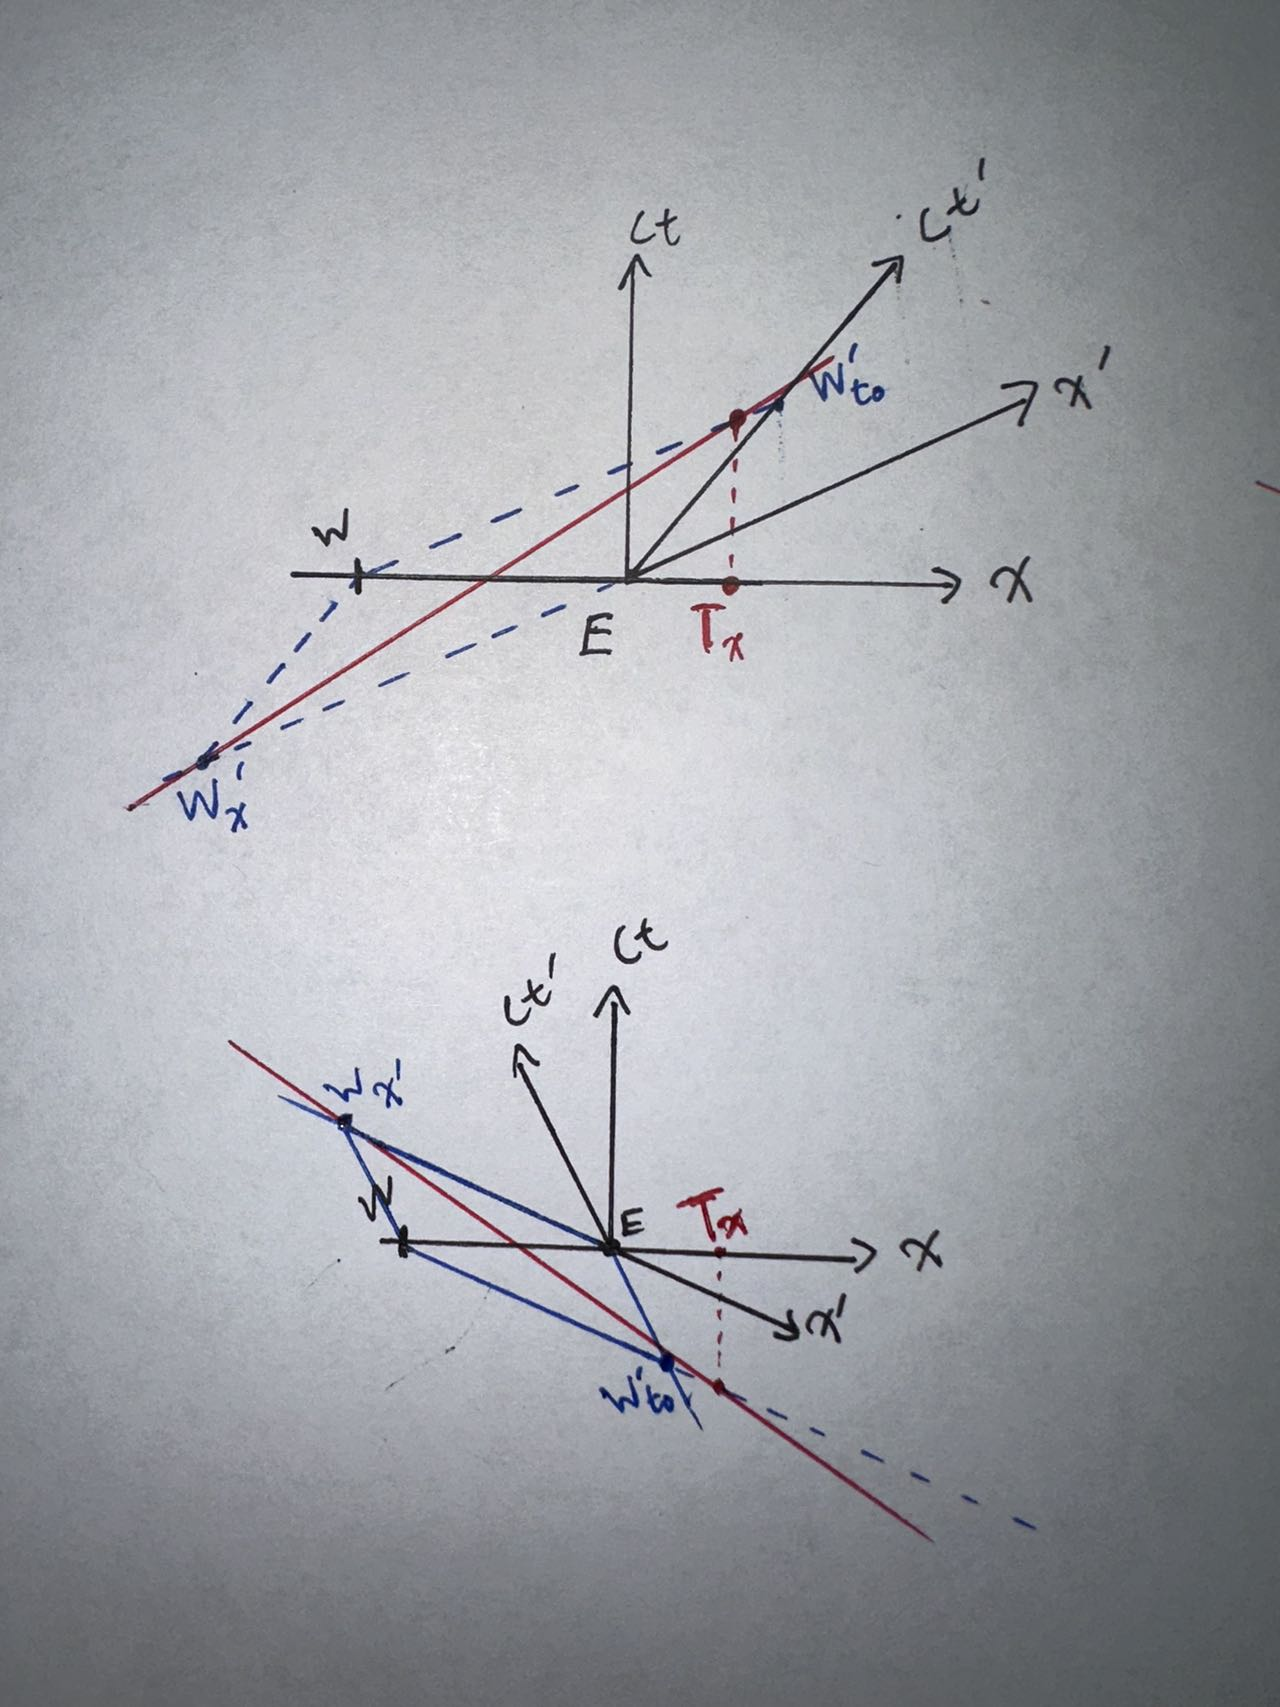
\includegraphics[scale = 0.22]{fig/Phys225_HW4_fig1.jpeg}
        \end{figure}
    \end{itemize}
        \newpage
    \item [2.]\(\gamma_1 = \frac{1}{\sqrt{1-v_1^2/c^2}},\ \gamma_2 = \frac{1}{\sqrt{1-v_2^2/c^2}}\), \(\beta_1  = \frac{v_1}{c}, \ \beta_1  = \frac{v_1}{c}\).

                \[\begin{bmatrix} 
                        \frac{1}{\sqrt{1-v_1^2/c^2}}& \frac{v_1}{\sqrt{c^2-v_1^2}}\\
                        \frac{v_1}{\sqrt{c^2-v_1^2}}& \frac{1}{\sqrt{1-v_1^2/c^2}}
                \end{bmatrix}
                \begin{bmatrix}
                    \frac{1}{\sqrt{1-v_2^2/c^2}}& \frac{v_2}{\sqrt{c^2-v_2^2}}\\
                    \frac{v_2}{\sqrt{c^2-v_2^2}}& \frac{1}{\sqrt{1-v_2^2/c^2}}
                \end{bmatrix}\]\[=
                \begin{bmatrix}
                    \frac{1}{\sqrt{(1-v_1^2/c^2)(1-v_2^2/c^2)}}+\frac{v_1v_2}{\sqrt{(c^2-v_1^2)(c^2-v_2^2)}}&
                    \frac{v_2}{\sqrt{(1-v_1^2/c^2)(c^2-v_2^2)}}+\frac{v_1}{\sqrt{(1-v_2^2/c^2)(c^2-v_1^2)}}
                    \\ \cdots&\cdots
                \end{bmatrix}\]
                Thus, \[\beta = \gamma \beta / \gamma\]
                \[=\frac{v_2\sqrt{(1-v_2^2/c^2)(c^2-v_1^2)}+v_1\sqrt{(1-v_1^2/c^2)(c^2-v_2^2)}}{\sqrt{(c^2-v_1^2)(c^2-v_2^2)}+v_1v_2\sqrt{(1-v_1^2/c^2)(1-v_2^2/c^2)}}\]
                Thus, \(v = \beta \times c\)
                \begin{align*}
                    &=\frac{v_2\sqrt{(1-v_2^2/c^2)(c^2-v_1^2)}+v_1\sqrt{(1-v_1^2/c^2)(c^2-v_2^2)}}{\sqrt{(c^2-v_1^2)(c^2-v_2^2)}+v_1v_2\sqrt{(1-v_1^2/c^2)(1-v_2^2/c^2)}}
                    \times c\\&=\frac{v_2\sqrt{(c^2-v_2^2)(c^2-v_1^2)}+v_1\sqrt{(c^2-v_1^2)(c^2-v_2^2)}}{\sqrt{(c^2-v_1^2)(c^2-v_2^2)}+v_1v_2\sqrt{(1-v_1^2/c^2)(1-v_2^2/c^2)}}
                    \\&=\frac{\sqrt{(c^2-v_2^2)(c^2-v_1^2)}(v_1+v_2)}{\sqrt{(c^2-v_1^2)(c^2-v_2^2)}+v_1v_2\sqrt{(1-v_1^2/c^2)(1-v_2^2/c^2)}}
                    \\&=\frac{v_1+v_2}{1+v_1v_2\sqrt{\frac{(1-v_1^2/c^2)(1-v_2^2/c^2)}{(c^2-v_2^2)(c^2-v_1^2)}}}
                    \\&=\frac{v_1+v_2}{1+v_1v_2\sqrt{\frac{(1-v_1^2/c^2)(1-v_2^2/c^2)}{(1-v_2^2/c^2)c^2(1-v_1^2/c^2)c^2}}}
                    \\&=\frac{v_1+v_2}{1+v_1v_2/c^2}
                \end{align*}
\end{itemize}


\end{document}